\documentclass[tikz,border=10pt]{standalone}
\usepackage{tikz}
\usetikzlibrary{
    positioning,
    shapes.geometric,
    shapes.multipart,
    arrows.meta,
    calc,
    fit,
    backgrounds,
    decorations.pathreplacing,
    patterns,
    matrix
}

% Color scheme matching AMICI paper style
\definecolor{receivercolor}{RGB}{255, 165, 0}   % Orange - receiver (center)
\definecolor{ringcolor}{RGB}{60, 179, 113}      % Green - spatial rings
\definecolor{hlcacolor}{RGB}{70, 130, 180}      % Steel blue - healthy reference
\definecolor{lucacolor}{RGB}{205, 92, 92}       % Indian red - cancer reference
\definecolor{pathwaycolor}{RGB}{147, 112, 219}  % Purple - pathway token
\definecolor{statscolor}{RGB}{100, 100, 100}    % Gray - stats token
\definecolor{attncolor}{RGB}{255, 215, 0}       % Gold - attention

\begin{document}
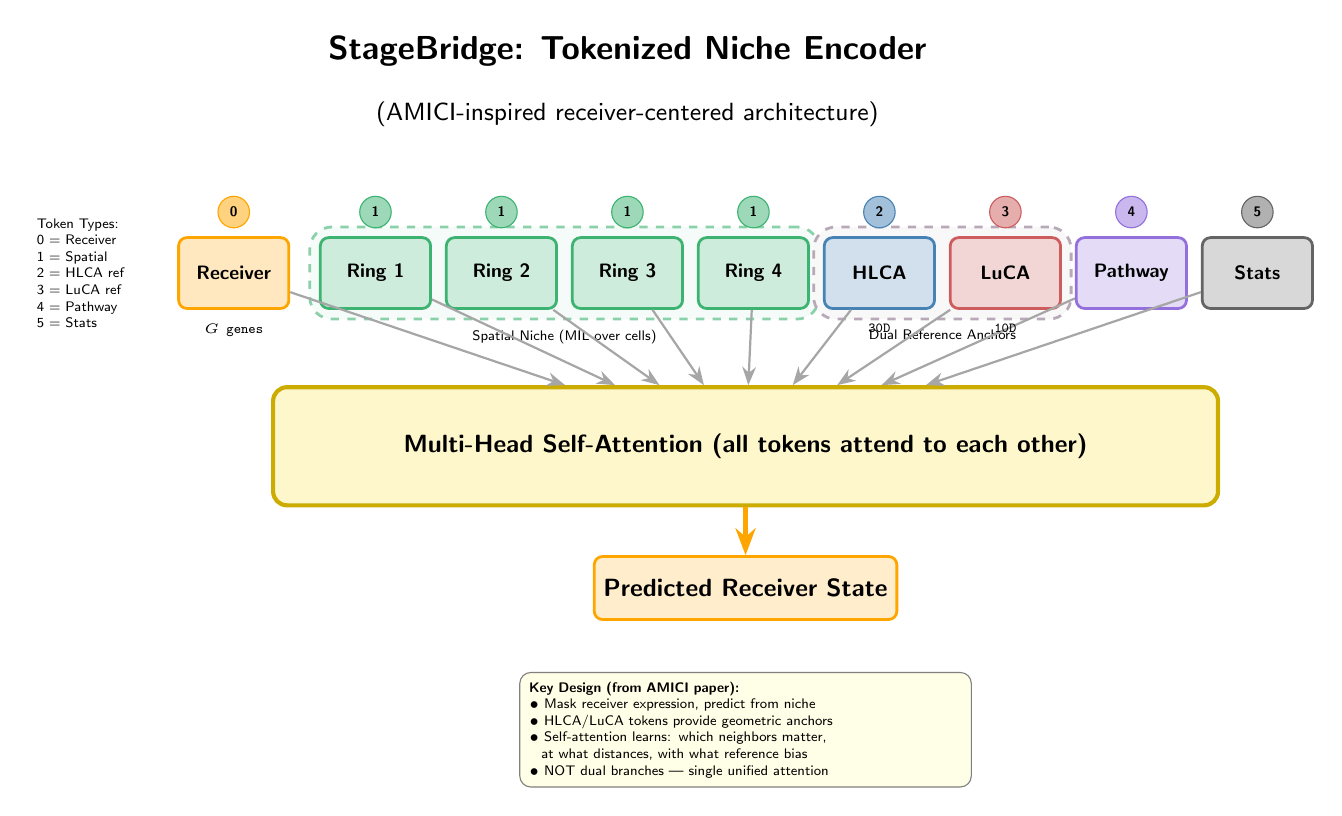
\begin{tikzpicture}[
    % Token styles
    token/.style={
        rectangle,
        draw=#1,
        fill=#1!25,
        rounded corners=3pt,
        minimum width=1.4cm,
        minimum height=0.9cm,
        font=\scriptsize\sffamily\bfseries,
        line width=1pt
    },
    % Type indicator
    typelabel/.style={
        circle,
        draw=#1,
        fill=#1!50,
        minimum size=0.4cm,
        font=\tiny\sffamily\bfseries,
        inner sep=1pt
    },
    % Attention block
    attnblock/.style={
        rectangle,
        draw=attncolor!80!black,
        fill=attncolor!20,
        rounded corners=5pt,
        minimum width=12cm,
        minimum height=1.5cm,
        font=\small\sffamily\bfseries,
        line width=1.5pt
    },
    % Output style
    output/.style={
        rectangle,
        draw=receivercolor,
        fill=receivercolor!20,
        rounded corners=3pt,
        minimum width=2.5cm,
        minimum height=0.8cm,
        font=\small\sffamily\bfseries,
        line width=1pt
    },
    % Arrow style
    arrow/.style={
        ->,
        >=Stealth,
        line width=0.8pt,
        #1
    },
    % Dashed group
    groupbox/.style={
        rectangle,
        draw=#1!60,
        fill=#1!5,
        rounded corners=8pt,
        dashed,
        line width=1pt
    }
]

% Title
\node[font=\large\sffamily\bfseries, anchor=south] at (0, 5.5)
    {StageBridge: Tokenized Niche Encoder};
\node[font=\small\sffamily, anchor=north] at (0, 5.3)
    {(AMICI-inspired receiver-centered architecture)};

% ============================================
% 9-TOKEN SEQUENCE
% ============================================

% Receiver token (center, type 0)
\node[token=receivercolor] (recv) at (-5, 3) {Receiver};
\node[typelabel=receivercolor, above=0.1cm of recv] {0};

% Ring tokens (spatial niche, type 1)
\node[token=ringcolor] (ring1) at (-3.2, 3) {Ring 1};
\node[typelabel=ringcolor, above=0.1cm of ring1] {1};

\node[token=ringcolor] (ring2) at (-1.6, 3) {Ring 2};
\node[typelabel=ringcolor, above=0.1cm of ring2] {1};

\node[token=ringcolor] (ring3) at (0, 3) {Ring 3};
\node[typelabel=ringcolor, above=0.1cm of ring3] {1};

\node[token=ringcolor] (ring4) at (1.6, 3) {Ring 4};
\node[typelabel=ringcolor, above=0.1cm of ring4] {1};

% Reference tokens (dual anchors)
\node[token=hlcacolor] (hlca) at (3.2, 3) {HLCA};
\node[typelabel=hlcacolor, above=0.1cm of hlca] {2};

\node[token=lucacolor] (luca) at (4.8, 3) {LuCA};
\node[typelabel=lucacolor, above=0.1cm of luca] {3};

% Auxiliary tokens
\node[token=pathwaycolor] (path) at (6.4, 3) {Pathway};
\node[typelabel=pathwaycolor, above=0.1cm of path] {4};

\node[token=statscolor] (stats) at (8, 3) {Stats};
\node[typelabel=statscolor, above=0.1cm of stats] {5};

% Token type legend
\node[font=\tiny\sffamily, text width=2cm, align=left] at (-6.5, 3) {
    Token Types:\\
    0 = Receiver\\
    1 = Spatial\\
    2 = HLCA ref\\
    3 = LuCA ref\\
    4 = Pathway\\
    5 = Stats
};

% ============================================
% SELF-ATTENTION BLOCK
% ============================================

\node[attnblock] (attn) at (1.5, 0.8) {Multi-Head Self-Attention (all tokens attend to each other)};

% Connections from tokens to attention
\foreach \tok in {recv, ring1, ring2, ring3, ring4, hlca, luca, path, stats} {
    \draw[arrow=gray!70] (\tok) -- (attn);
}

% ============================================
% OUTPUT LAYER
% ============================================

\node[output] (out) at (1.5, -1) {Predicted Receiver State};

\draw[arrow=receivercolor, line width=1.5pt] (attn) -- (out);

% ============================================
% ANNOTATIONS
% ============================================

% Spatial niche grouping
\begin{scope}[on background layer]
    \node[groupbox=ringcolor, fit=(ring1)(ring2)(ring3)(ring4),
          label={[font=\tiny\sffamily]below:Spatial Niche (MIL over cells)}] {};

    \node[groupbox=hlcacolor!50!lucacolor, fit=(hlca)(luca),
          label={[font=\tiny\sffamily]below:Dual Reference Anchors}] {};
\end{scope}

% Key insight box
\node[rectangle, draw=black!50, fill=yellow!10, rounded corners,
      font=\tiny\sffamily, text width=5.5cm, align=left] at (1.5, -2.8) {
    \textbf{Key Design (from AMICI paper):}\\
    $\bullet$ Mask receiver expression, predict from niche\\
    $\bullet$ HLCA/LuCA tokens provide geometric anchors\\
    $\bullet$ Self-attention learns: which neighbors matter,\\
    \hspace{0.5em} at what distances, with what reference bias\\
    $\bullet$ NOT dual branches --- single unified attention
};

% Dimension annotations
\node[font=\tiny\ttfamily, below=0.05cm of recv] {$G$ genes};
\node[font=\tiny\ttfamily, below=0.05cm of hlca] {30D};
\node[font=\tiny\ttfamily, below=0.05cm of luca] {10D};

\end{tikzpicture}
\end{document}
